\documentclass[paper=a4,fontsize=12pt,DIV=calc]{scrreprt}
\usepackage[utf8]{inputenc}
\usepackage[T1]{fontenc}
\usepackage{lmodern}
\usepackage[english,french]{babel}
\usepackage[babel]{csquotes}
\MakeAutoQuote{«}{»}	

\usepackage[a4paper, pass]{geometry}
\usepackage{graphicx}
\usepackage{xcolor}
\usepackage{multicol}
\usepackage{setspace}
\usepackage[colorlinks=true, urlcolor=blue]{hyperref}

\usepackage{tikz}
\usetikzlibrary{decorations.markings}
\definecolor{blueamu}{RGB}{0, 101, 189}
\definecolor{cyanamu}{RGB}{61, 183, 228}
\newcommand{\dhorline}[3][0]{%
    \tikz[baseline=-2pt]{\path[decoration={markings, 
      mark=between positions 0 and 1 step 2*#3
      with {\node[color=blueamu, fill, circle, minimum width=#3, inner sep=0pt, anchor=south west] {};}},postaction={decorate}]  (0,#1) -- ++(#2,0);}}
\newcommand{\dvertline}[3][0]{%
    \tikz[baseline=2em]{\path[decoration={markings,
      mark=between positions 0 and 1 step 2*#2
      with {\node[color=black!50, fill, circle, minimum width=#2, inner sep=0pt, anchor=south west] {};}},postaction={decorate}] (0, #1) -- ++(0,#3);}}  

\graphicspath{{fig/}{logo/}}

\newcommand\titel[1]{{\usefont{T1}{tit}{el}{n} #1 }}
\newcommand\titl[1]{{\usefont{T1}{tit}{l}{n} #1 }}
\newcommand\titm[1]{{\usefont{T1}{tit}{m}{n} #1 }}
\newcommand\titsb[1]{{\usefont{T1}{tit}{sb}{n} #1 }}
\newcommand\titb[1]{{\usefont{T1}{tit}{b}{n} #1 }}
\makeatletter\newcommand\HUGE{\@setfontsize\Huge{28}{0}}\makeatother

\usepackage{lipsum}

\begin{document}
    \newgeometry{margin=2em}
    \newgeometry{margin=2em}

\begin{center}
	\begin{minipage}[c]{.5\linewidth}
		\raggedright
\includegraphics[height=7em]{logo_amu_excellence}
	\end{minipage}\hfill
	\begin{minipage}[c]{.5\linewidth}
		%\raggedleft\includegraphics[height=7em]{example-image-b} %% logo cotutelle
	\end{minipage}\hfill
\end{center}

\vspace{1em}

\begin{center}
	\begin{minipage}[c]{.63\linewidth}
		\dhorline{\textwidth}{4pt}
	\end{minipage}\hfill
	\begin{minipage}[c]{.35\linewidth}
		\raggedleft\titl{NNT/NL : 2020AIXM0001/001ED000}
		% renseigner votre numéro national de thèse (NNT) et le numéro local (NL)
		% ils sont indiqués sur la page d'informations administratives de votre espace de dépôt dans le guichet de dépôt légal des thèses AMU lorque votre date de soutenance est renseignée par votre service de scolarité
		% https://depot-theses.univ-amu.fr/
	\end{minipage}\hfill
\end{center}

%\vspace{1em}

\doublespacing
\begin{flushleft}
    \titb{\HUGE\textcolor{cyanamu}{THÈSE DE DOCTORAT}}\\
	\titl{\Large Soutenue à Aix-Marseille Université}\\
	%\titl{\Large dans le cadre d'une cotutelle avec }\\
	\titl{\Large le 10 janvier 2020 par}\\
\end{flushleft}
\vspace{2em}
\begin{center}
	\titsb{\Huge Prénom NOM}\\
    \vspace{1em}
	\titm{\LARGE Titre de la thèse:\\ sous-titre de la thèse}\\
\end{center}
\singlespacing

\vspace{4em}

\begin{center}
	\begin{minipage}[t]{.45\linewidth}
    	    \vspace{.5em}
        	\titb{Discipline}
        	
        	\titl{renseigner la discipline du doctorat}
        	
    	    \vspace{1em}
        	\titb{Spécialité}
        	
        	\titl{renseigner la spécialité du doctorat}
        	
    	    \vspace{2em}
        	\titb{École doctorale}
        	
        	\titl{renseigner l'école doctorale}
        	
    	    \vspace{1em}
        	\titb{Laboratoire/Partenaires de recherche}
        	
        	\titl{renseigner les partenaires institutionnels
        	
        	et les partenaires privés
        	
        	un partenaire par ligne
        	}
	\end{minipage}\hfill
	\begin{minipage}[t]{.03\linewidth}
	    \dvertline{4pt}{-16em}
	\end{minipage}\hfill
	\begin{minipage}[t]{.52\linewidth}
	    \vspace{.5em}
    	\titb{\small Composition du jury}

	    \vspace{1em}
    	\titel{
        \begin{tabular}{p{12em} p{9.5em}}
        	Prénom NOM & Rapporteur·e \\
        	Affiliation \\
        	\\
        	Prénom NOM & Rapporteur·e \\
        	Affiliation \\
            \\
            Prénom NOM & Examinateur·rice \\
        	Affiliation \\
            \\
        	Prénom NOM & Président·e du jury \\
        	Affiliation \\
            \\
        	Prénom NOM & Directeur·rice de thèse \\
        	Affiliation \\
        \end{tabular}
        }
	\end{minipage}\hfill
\end{center}       

\vspace{2em}

\begin{center} %% logos partenaires
	\begin{minipage}[c]{.25\linewidth}
		\centering\includegraphics[height=5em]{example-image-a} 
	\end{minipage}\hfill
	\begin{minipage}[c]{.25\linewidth}
		\centering\includegraphics[height=5em]{example-image-b}
	\end{minipage}\hfill
	\begin{minipage}[c]{.25\linewidth}
		\centering\includegraphics[height=5em]{example-image-c} 
	\end{minipage}\hfill
	\begin{minipage}[c]{.25\linewidth}
		\centering\includegraphics[height=5em]{example-image-c}
	\end{minipage}\hfill
\end{center}

\restoregeometry
    \restoregeometry
    \newgeometry{bottom=10em}

    \iftrue % Déclaration sur l'honneur pour une thèse en français (inverser les \if pour une thèse en anglais)
    Je soussigné, [Prénom Nom], %% Prénom et Nom de l'auteur %%
    déclare par la présente que le travail présenté dans ce manuscrit est mon propre travail, réalisé sous la direction scientifique de [Prénom Nom], % Prénom et Nom du directeur de thèse et s’il y a lieu du co-directeur de thèse
    dans le respect des principes d’honnêteté, d'intégrité et de responsabilité inhérents à la mission de recherche. Les travaux de recherche et la rédaction de ce manuscrit ont été réalisés dans le respect à la fois de la charte nationale de déontologie des métiers de la recherche et de la charte d’Aix-Marseille Université relative à la lutte contre le plagiat.
    
    Ce travail n'a pas été précédemment soumis en France ou à l'étranger dans une version identique ou similaire à un organisme examinateur.\\
    
    Fait à [ville] le [date]
    
    \begin{flushright}\includegraphics[width=120px,height=40px]{example-image-a}\end{flushright}% signature
\fi

\iffalse % Affidavit of Honour for english thesis (invert the \if for an English thesis)
    I, undersigned, [First Name Surname], %% First Name and Surname of the PhD student
    hereby declare that the work presented in this manuscript is my own work, carried out under the scientific direction of [First Name Surname], %% First Name and Surname of the thesis director and if applicable of the co-thesis director
    in accordance with the principles of honesty, integrity and responsibility inherent to the research mission. The research work and the writing of this manuscript have been carried out in compliance with both the french national charter for Research Integrity and the Aix-Marseille University charter on the fight against plagiarism.
    
    This work has not been submitted previously either in this country or in aother country in the same or in a similar version to any other examination body.\\
    
    [Place] [date]
    
    \begin{flushright}\includegraphics[width=120px,height=40px]{example-image-b}\includegraphics[width=40,height=15px]{example-image-a}\end{flushright} % signature
\fi

~\vfill
\begin{center}
	\begin{minipage}[c]{0.25\linewidth}
		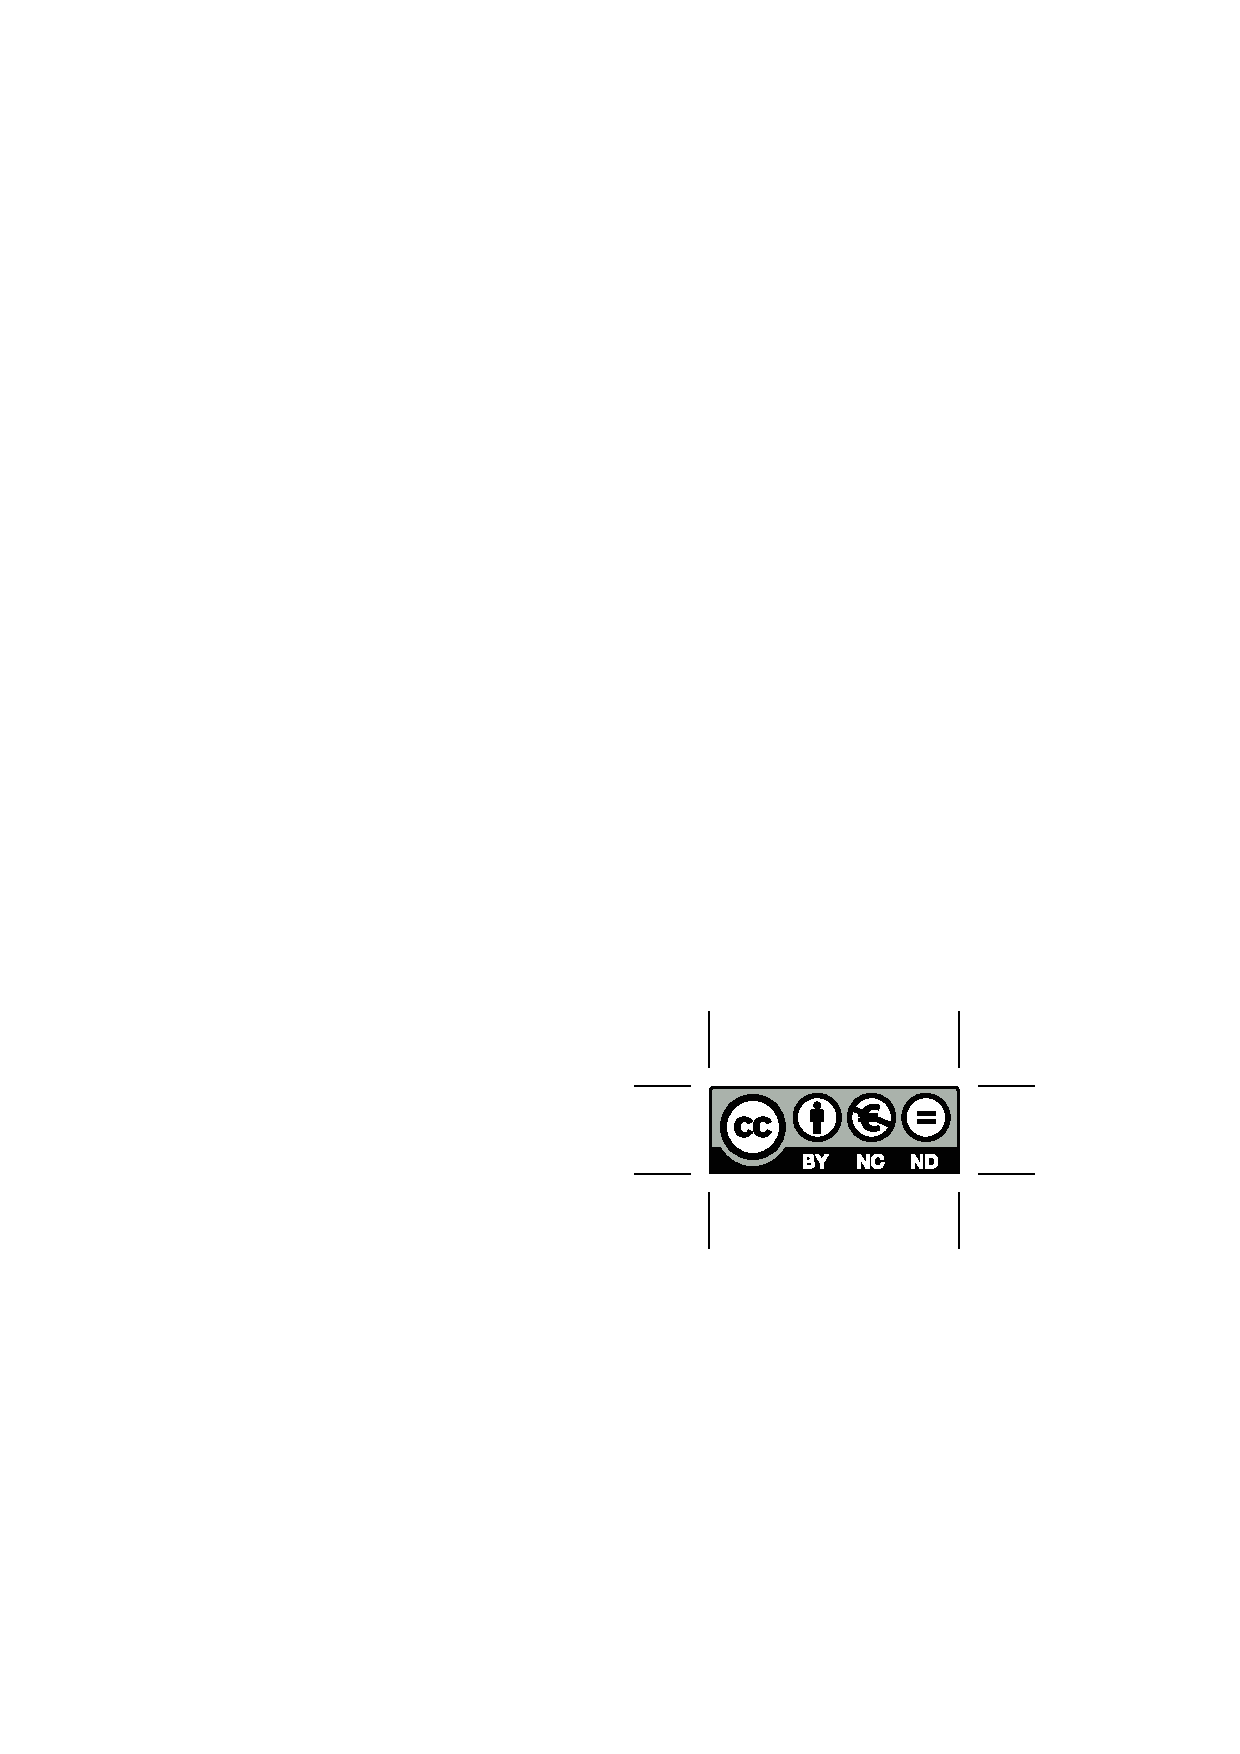
\includegraphics[height=35px]{by-nc-nd-eu}
	\end{minipage}\hfill
\end{center}

Cette \oe{}uvre est mise à disposition selon les termes de la \href{https://creativecommons.org/licenses/by-nc-nd/4.0/deed.fr}{Licence Creative Commons Attribution - Pas d’Utilisation Commerciale - Pas de Modification 4.0 International}. % consultez les conditions de la licence cc by-nc-nd, vous pouvez appliquer une licence moins restrictive, cc by-nc-sa par exemple

  \chapter*{Liste de publications et participation aux conférences}
    \subsection*{Liste des publications réalisées dans le cadre du projet de thèse:}
\begin{enumerate}
\item 
\item 
\item 
\end{enumerate}


\subsection*{Participation aux conférences et écoles d’été au cours de la période de thèse:}
\begin{enumerate}
\item 
\item 
\item 
\end{enumerate}
	\chapter*{Résumés}
    \lipsum[1]\index{Lorem ipsum}

\vspace{0.5cm}
Mots clés: géométrie algorithmique, complexe planaire et rectangulaire, géodésique, courbure globale non-positive



  \chapter*{Abstract}
    \selectlanguage{english}
    \selectlanguage{english}

\lipsum[1]\index{Lorem ipsum}

\vspace{0.5cm}
Keywords: computational geometry, planar and rectangular complex, geodesic, global nonpositive curvature

\selectlanguage{french}

    \selectlanguage{french}

\end{document}